% The \phantomsection command is needed to create a link to a place in the document that is not a
% figure, equation, table, section, subsection, chapter, etc.
%
% When do I need to invoke \phantomsection?
% https://tex.stackexchange.com/questions/44088/when-do-i-need-to-invoke-phantomsection
\phantomsection


% Multiple-language document - babel - selectlanguage vs begin/end{otherlanguage}
% https://tex.stackexchange.com/questions/36526/multiple-language-document-babel-selectlanguage-vs-begin-endotherlanguage
\begin{otherlanguage*}{brazil}

    \chapter{Pesquisa}

    \begin{flushright}
         
    \end{flushright}


    % \newpage

    \section{Início da Pesquisa}

    Tendo pesquisado extensivamente tecnologias para web durante o mestrado, o desenvolvimento do trabalho em homenagem a Gilberto Gil, aliado ao surgimento do HTML5 e das tecnologias de web audio me apontaram para uma possibilidade concreta de dar prosseguimento às minhas pesquisas acadêmicas na área da música, e a experiência com o hexagrama mostrou que havia muita possibilidade na utilização criativa dessas novas tecnologias. 

Antes do HTML5, tudo que envolvia processamento de áudio em tempo real em páginas de internet era embasada em softwares proprietários como o Flash, ou plugins programados em alguma linguagem de baixo nível como Java, Python ou C++. O HTML5, junto com a WebAudio API, que estabelece parâmetros para processamento de áudio em JavaScript, permite que agora seja possível o controle de processos de áudio diretamente pelos navegadores, sem a necessidade de instalação de nenhum programa adicional. Um site como o Radio.garden, que mencionamos na introdução deste trabalho, possui uma interface que só é possível graças ao desenvolvimento dessas novas tecnologias de \emph{streamming} de áudio e geoprocessamento em 3D via JavaScript, que faz com que o grosso do processamento aconteça no computador do usuário, e não no servidor, diminuindo os custos com hospedagem.

Nossa hipótese era que utilizando essas tecnologias, poderíamos criar instrumentos musicais que explorassem possibilidades de inter-relação audiovisuais, acessíveis e que possam funcionar em qualquer computador que tenha instalado um navegador que suporte esses novos recursos, podendo funcionar inclusive localmente em máquinas sem acesso à internet e dispositivos móveis. Partíamos da ideia de que seria possível utilizar criativamente essas tecnologias para propor novas interfaces para expressão musical.
    
A ideia inicial, era trabalhar em alguns projetos de instrumentos musicais, que pudessem ser usados por qualquer um para compor ou performar música eletrônica. Desde o início, ficou claro que essa pesquisa tinha um caráter bastante interdisciplinar, partindo do design, mas abarcando questões como interação humano computador (IHC), semiótica, computação musical, música experimental, filosóficas e políticas. 

\subsubsection{Interface como pesquisa}
A interface é considerada pelo campo de estudos de IHC, como “uma fronteira através da qual dois sistemas se comunicam (o humano e o programa)” (Magnussom, 2005), ou a parte visível de um sistema complexo, método ou classe, segundo a definição da engenharia de software, uma base de controle simples e inteligível que permite às pessoas um controle de alto nível sobre estruturas subjacentes. Ela pode ser considerada um sistema de comunicação, pois “conecta dois agentes e objetos” criando “um espaço sígnico comum a esses agentes” (IAZZETTA, 1997: 105). Ao mesmo tempo que ela permite que uma pessoa comunique certas coisas a um software, por exemplo, ela também é o que comunica coisas à pessoa sobre o software. Magnusson (2005 p. 212) defende que a própria interface pode ser vista como uma ideologia musical: 

\begin{citacao}
A interface é um instrumento. É uma manifestação gráfica de ideias musicais e processos de trabalho. A interface é ao mesmo tempo a plataforma estética definindo as estruturas musicais e a base prática de controle para o sistema sonoro subjacente. De um certo modo pode ser vista como uma ideologia musical. Ela define possibilidades, mas também define as limitações do que pode ser composto ou tocado. Aqui nós estamos pensando principalmente nas interfaces gráficas de softwares de áudio, mas esse argumento pode ser estendido às linguagens de programação de áudio também: os objetos e classes pré-programados à disposição em uma dada linguagem definem o que pode ser expressado. (tradução nossa)
\end{citacao}

Uma grande referência no campo de pesquisa do design de interfaces é Douglas Engelbarth, que com o trabalho no Augmentation Research Center (ARC), deu origem a uma série de desenvolvimentos fundamentais nas interfaces para computadores. Foi lá que foram desenvolvidos os primeiros editores de texto, o mouse e o conceito de espaço visual no computador, entre outros recursos que foram fundamentais na história da computação. O trabalho do laboratório, que desencadeou em mudanças radicais em todas tecnologias posteriores era baseado em uma metodologia que chamavam de \emph{bootstrapping}, que se tratava basicamente em buscar construir ferramentas para o próprio trabalho, no caso, o de programação dos computadores compartilhados da época. Em 1962, as companhias já tinham desenvolvido o computador, que era ainda utilizado principalmente para ferramentas militares, e eram grandes máquinas compartilhadas com interface mediada somente por texto. A pesquisa deles procurava desenvolver o potencial do computador como ferramenta para ampliação do intelecto humano \cite{Engelbart1962}.

O conceito de \emph{bootstraping} fez, de uma certa maneira, que eu mudasse o foco inicial da pesquisa, que era de construir coisas genéricas para um usuário genérico, como é tradicionalmente a metodologia do design, para procurar construir instrumentos que fossem acima de tudo, ferramentas para a nossa própria pesquisa prática em música experimental, individual e junto a redes como NuSom, Sonora, Tecnoxamanismo, BlóKõKê, Orquestra Errante entre outras.

Na história da música existe uma série de casos onde a ideia de desenvolver seus próprias tecnologias para produção sonora moveu parte da pesquisa dos músicos.

John and James whitney, por exemplo, considerados precursores da musica visual, criaram um sistema mecanizado, baseado em conjunto de pêndulos que capaz de escrever ondas senoidais na faixa de som, uma impressora sonora, como ele explica abaixo:

\begin{citacao}
Nosso instrumento de som subsônico consistia em uma série de pendulos ligados mecanicamente a uma cunha ótica. (...) Nenhum som audível era gerado pelo instrumento. Ao invés disso, uma trilha sonora ótica de dimensões padrão era sintéticamente exposta no filme, que depois de processado podia ser tocado em um projetor de filmes padrão."\cite[152]{Whitney1980} 
\end{citacao}

Com esse instrumento, os irmãos fizeram ``Five Abstract Film Exercises''. O resultado sonoro, que trazia ondas pura senoidais e até glissandos foram chocantes para época, e garantiu à dupla o prêmio pelo som na competição de filmes experimentais de Bruxelas de 1949.

Enquanto seu irmão James – assim como Fischinger – foi com o tempo passando a se voltar mais à pintura e a questões mísiticas e de espiritualidade, John procurou a se dedicar mais ao desenvolvimento tecnológico e a sistematizar um pensamento sobre música e linguagem visual. Ao longo dos anos ele foi desenvolvendo um computador mecânico analógico, especialmente para animação com tipografia de ``design concreto'' (Youngblood, 1970), prestando serviços para a indústria de filmes, assim como Fischinger. Ele colaborou com Saul Bass na famosa abertura para o filme Vertigo, de Hitchcock, por exemplo. Sua máquina era formada por câmeras e mecanismos rotativos capazes de produzir imagens em movimento no filme a partir de moldes de cartolina e cálculos matemáticos complexos. Era, na visão de Youngblood \cite{Youngblood1970}, ``um homem de amanhã no mundo de hoje''. Whitney usou como base para seu primeiro computador analálogico um dispositivo antimísseis M-5, ressignificando um equipamento militar, ou nas palavras de Youngblood, ``uma arma da morte'' em uma máquina capaz de produzir beleza.

Outra referência histórica importante é o trabalho de Daphne Oram, precursora da música eletrônica que desenvolveu um sintetizador de música baseado em desenhos. O Oramics funcionava através de desenhos que definiam envelope, e perfil melódico do som. Oram observou que a música eletrônica dital na época era regida principalmente por ``processos impositivos", principalmente baseados em tom, volume e duração, ou baseados em sons puros, como de osciladores, ou em desenhos de onda definidos digitalmente, que segundo ela ``tinham pouca finesse'' \cite[101]{Oram1972}: 

\begin{citacao}
One of the points to notice in digital computer music is the
quality of each note ... its timbre, its subtlety, its individual shape and phrasing. When you come to program your digital computer will you, mostly, be concerned with the regulation of pitch and rhythm and interval relationship? Will you be able to give time, also, to considering the beauty of each individual note... the subtleindividuality of each note ... as well as its place in the main scheme? Will each note, each phrase or melisma, be able to affirm the richness and the character of its own individuality, while it is taking its balanced position in the overall structure? 

We wish to design this machine-with-humanising-factors so that the composer can instruct it by means of a direct and simple language. He will want to transduce his thoughts as quickly as possible, via a channel which is logical. \cite[97]{Oram1972}
\end{citacao}

Seu desejo era de criar uma máquina em que ela pudesse desenhar os sons, e para tanto, ela passou muitos anos desenvolvendo a ideia dessa máquina até que conseguiu recursos para construí-la. 


\todo[inline]{
outras práticas da comunidade NIME
} 



\subsubsection{Interfaces gráficas para produção musical}

Nos primeiros computadores a interface era física e a programação era operada por meio de cabos e potenciômetros diretamente no nível do hardware, \cite[110]{Henrique1996}. O ENIAC (1943 - 1946) (figura 1), um dos primeiros computadores construídos durante a Segunda Guerra Mundial com fins militares \cite[24]{Stolfi}, era operado por pessoas com grau avançado de domínio da matemática, muitas das quais mulheres que já trabalhavam na guerra como computadoras fazendo manualmente cálculos de balística \cite{HayleyWilliams2015}, sua interface tem uma certa semelhança com a dos grandes sintetizadores modulares construídos anos depois, como o feito por Joseph Paradiso a partir de 1974, e que foi remontado em 2012 em uma exposição no MIT \ref{analogicos}. 

\begin{figure}[ht]
    \caption{\label{analogicos}À esquerda, interface do ENIAC, a programação era feita diretamente no nível do hardware, através de cabos e potenciômetros.  À direita o sintetizador modular montado por Joseph Paradiso, um dos maiores, montado no museu do MIT de janeiro a abril de 2012.}
    \begin{center}
        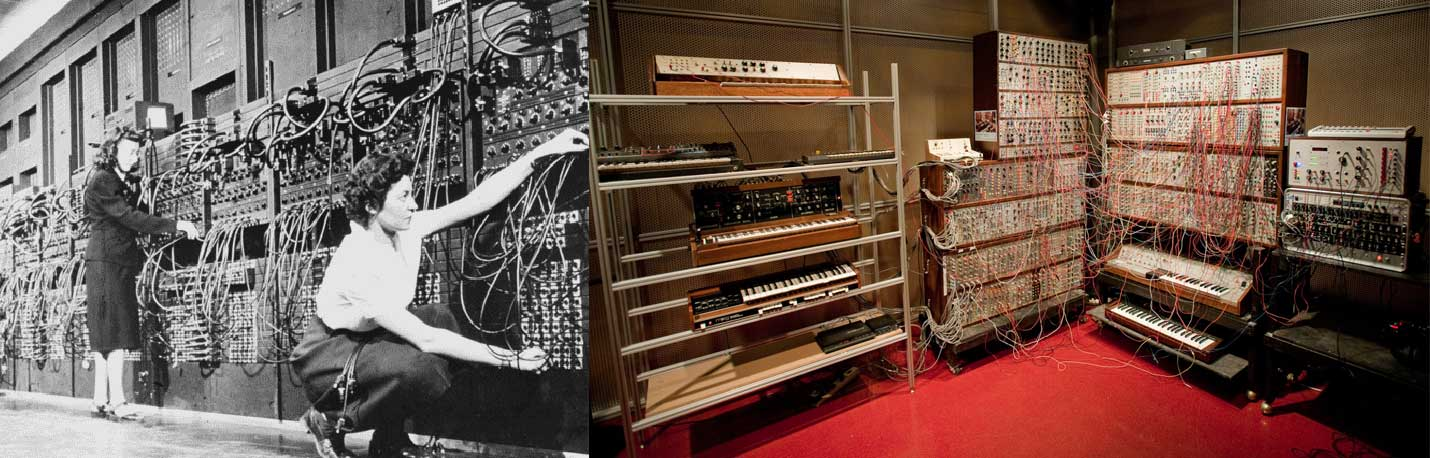
\includegraphics[width=1\linewidth]{pictures/analogicos}
    \end{center}
    \legend{Fonte: \cite{HayleyWilliams2015} e http://web.media.mit.edu/~joep/pics/ FullSynthMIT-Museum.jpg}
\end{figure}

As primeiras experiências musicais em computadores digitais foram realizadas na década de 50 por Max Mathews no Bell Telecom Lab. Para gerar os primeiros sons computadorizados, Max teve que desenvolver uma linguagem de programação própria, que chamou de \emph{Music I} \cite[253]{Holmes1985}. Depois de uma década desenvolvendo essa linguagem de programação musical, em 1968 passou a trabalhar no desenvolvimento do GROOVE ou \emph{General Real-time Output Operations on Voltage-controlled Equipment}, um equipamento que funcionava na plataforma \emph{Graphic 1}, ``um sistema computadorizado interativo que podia traduzir imagens desenhadas com uma caneta luminosa em uma tela'' \cite[253]{Holmes1985}, que era similar à plataforma utilizada por Ivan Sutherland no \emph{Sketchpad}. O GROOVE teve a primeira interface gráfica interativa para computação musical. 

\begin{figure}[ht]
    \caption{\label{max}Max Mathews e L. Rosler com a estação de trabalho Graphic 1. }
    \begin{center}
        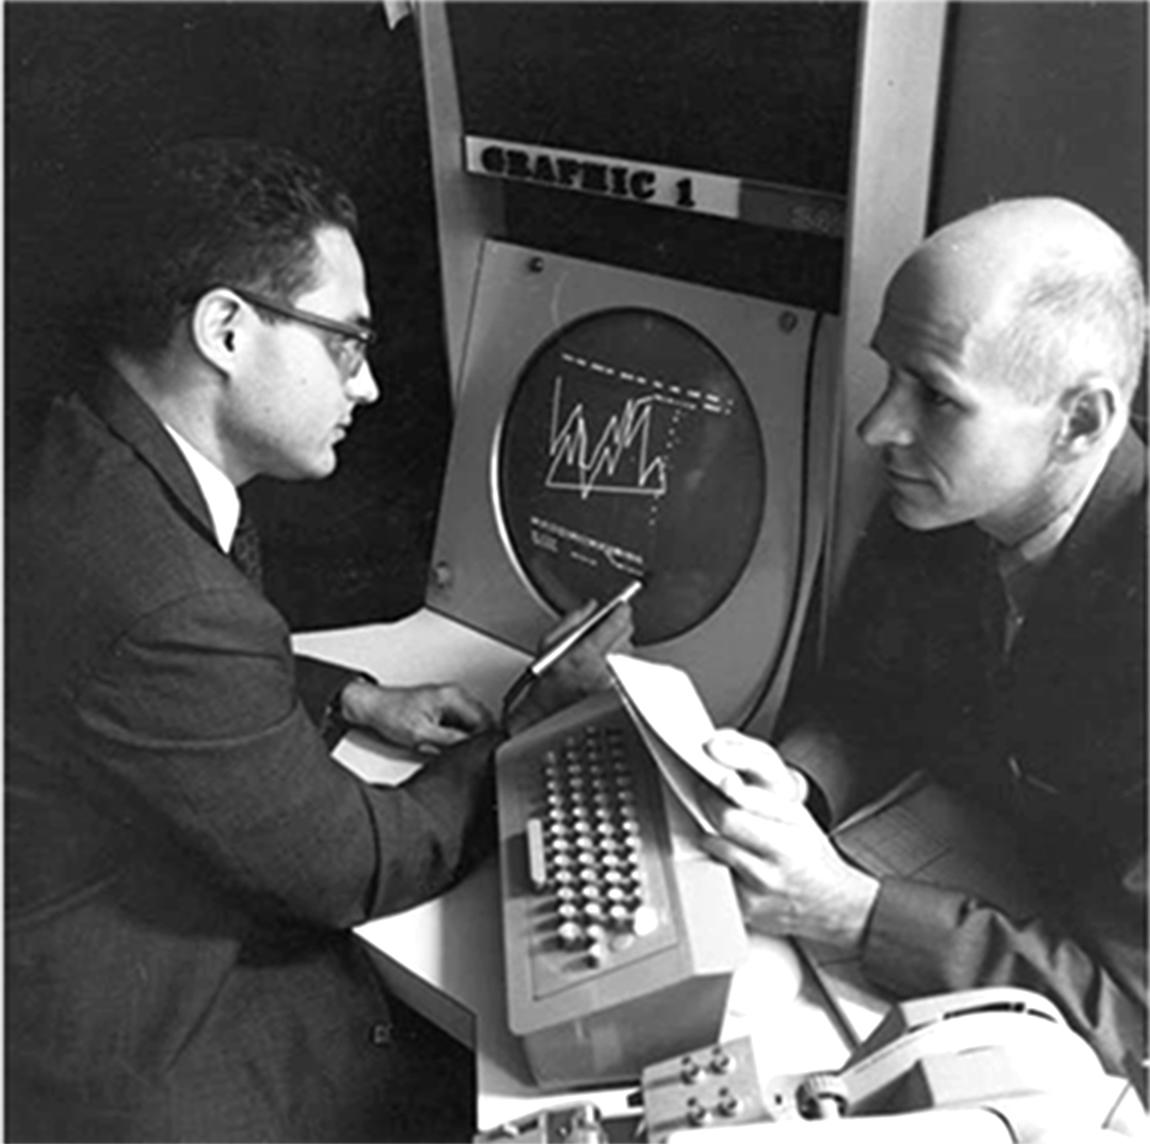
\includegraphics[width=0.5\linewidth]{pictures/MaxHolmes-251}
    \end{center}
    \legend{Fonte: Holmes, 1985 p. 251}
\end{figure}

Com o desenvolvimento da computação surgiram também novas formas de interação, como a alimentação e impressão de dados através de cartões perfurados e posteriormente o teletipo, um terminal parecido com o teclado dos computadores atuais, além da impressão de dados em tela por meio do tubo de raios catódicos. Com elas, a operação do computador não acontece mais no nível do hardware, e são desenvolvidas ``linguagens de programação mais eficiente e acessíveis'' (IAZZETTA, 1997 : 111). As próprias linguagens são interfaces que permitem a interação do programador com processos da máquina em um estágio mais bruto.

Até o final da década de 70, compositores precisavam trabalhar diretamente com programadores para realizar qualquer tipo de trabalho em computação musical. Foi o caso de James Tenney, que trabalhou com Mathews no Bell Telecom Lab para a composição de 6 peças ou o caso de Yannis Xenakis, que compôs \emph{Metastasis} quando teve acesso aos laboratórios da IBM em Paris\cite{Holmes1985}. Curtis Abbott, que escreveu o software da máquina 4C utilizada no final da década de 70 pelo IRCAN, começa seu artigo Music System Programming afirmando enfaticamente que ``programar é necessário para fazer qualquer coisa realmente nova em música computadorizada" \cite[51]{Roads1996}. A computação musical é um das vertentes desse campo que desponta na produção artística moderna, que Abbot já define como ``programação criativa'', um campo da computação que vai lidar com questões artísticas e estéticas. 

Na metade da década de 70, A New England Digital Corp. lançou comercialmente o primeiro sintetizador digital portátil, o Synclavier \cite[265]{Holmes1985}, com a interface que havia se tornado dominante entre os sintetizadores analógicos que dominavam o mercado, o teclado similar ao do piano \cite{JosephParadiso1998}. Com ele, a síntese digital era possível de ser acessada diretamente pelos músicos, através de sua interface familiar, mas apesar disso, seu preço na época estava entre \$200.000 e \$300.000 dólares, o que o tornava extremamente proibitivo. No começo da década de 80, já havia sido lançado também um sistema concorrente, o Fairlight CMI, que consistia em um sistema de processamento computadorizado, um monitor com caneta luminosa (lightpen), um teclado alfanumérico QWERTY, um teclado de 6 oitavas, além de um sistema de síntese analógica com 6 osciladores.

O Fairlight, apesar de mais acessível do que o Synclavier, era também um instrumento caro. Na época de seu lançamento o CMI original custava a partir de \$16.000 libras, o que não impediu que músicos famosos como Peter Gabriel, Kate Bush, Queen, Stevie Wonder, Herbie Hancock, Kraftwerk, Grace Jones, Frankie Goes To Hollywood, Thompson Twins, Human League, Tears for Fears entre outros o adotassem. \cite[18]{Twyman2004}(LEETE, 1999 e TWYMAN, 2004 : 18) O CMI era uma ferramenta atrativa tanto para engenheiros da computação, pelo processador sofisticado, quanto para compositores, que podiam utilizá-lo para fazer orquestração complexa de suas peças, quanto para músicos, que podiam utilizá-lo em estúdio ou em performances ao vivo. Mas não era uma ferramenta tão simples de se operar como anunciava. \cite[55]{Twyman2004}

Desde o lançamento do primeiro Macintosh, que tinha uma interface gráfica mais amigável, uma gama de softwares para a produção musical floresceu, voltadas para profissionais de música, desenvolvimento de jogos e performers. Em 1990, uma parceria entre a Digidesign, uma empresa que já desenvolvia softwares para produção musical e a Opcode, que era a maior fabricante de interfaces MIDI na década de 80 gerou o Studio Vision, que podia ser comprado por \$950 dólares e foi o primeiro a integrar gravação e edição de áudio e MIDI, sendo considerado o primeiro software do tipo digital audio workstation (DAW). Sua interface gráfica misturava conceitos desenvolvidos nos primeiros editores de áudio, como a representação do som através dos gráficos de amplitude por tempo, com um piano-roll, para marcação de notas em função do tempo. Isso ajudou a aproximar músicos que usavam editores de partitura digitais \cite{ChrisHalaby2011}. A interface de edição multipista permite gravar várias faixas e sobrepô-las paralelamente no espaço gráfico da tela, o que dá ao produtor musical a possibilidade de organização visual do fluxo sonoro ao longo do tempo, permitindo ajustes mais precisos de sincronização e mixagem.

No começo da década de 90, a tecnologia de gravação em disco rígido era extremamente cara e limitada, e as grandes empresas que dominavam o mercado de gravação em fita como a OTARI e a TASCAM não acreditavam que as pessoas iriam abandonar tão cedo as fitas magnéticas. Esse desinteresse permitiu que a Digidesign, que posteriormente veio se tornar a AVID, fosse se desenvolvendo continuamente e viesse a dominar o mercado de gravação digital até hoje, com as várias versões do Pro Tools que foram lançadas desde 1991 com sistemas integrados de hardware e software voltados para estúdios. Graças a uma placa de áudio que podia ser acoplada exteriormente ao Mac, o sistema de áudio permitia gravação multipista, processamento de sinal e sistema de mixagem sofisticados, que eram mais baratos que os sistemas de hardware disponíveis na época. (HALABY, 2011).

Para facilitar uma aproximação com os profissionais que já trabalhavam nos estúdios analógicos tradicionais, o sistema contava com uma interface gráfica de usuário que se apoiava na mímese do estúdio tradicional de gravação em fita. Assim, elementos familiares dos técnicos de estúdio foram copiados de uma maneira literal, sliders, displays luminosos, potenciômetros rotativos, botões de controle como play, pause e stop e somados ao modelo de interface de edição multipista desenvolvida no Studio Vision. 

Embora o discurso seja de uma revolução, na prática a interface se acomoda para ficar cada vez mais parecida ao estúdio tradicional. A cada versão do software lançada há um pequeno redesenho da interface gráfica, no sentido de acomodar mais recursos que são incluídos, mas também no sentido de tornar a interface mais “realista”, ou mais similar como imitação do estúdio de gravação analógica, com a inclusão de sombras, reflexos e degradés. Na figura abaixo, que mostra uma versão mais recente do software, podemos ver que os botões rotativos tem mais detalhes, como sombras e reflexos, e podemos ver também uma pequena tela similar à tela de um osciloscópio físico, que também possui um leve reflexo no canto superior esquerdo. Esses detalhes na prática não acrescentam nenhuma funcionalidade extra ao programa, na prática é possível que até prejudiquem, na medida que exigem gráficos mais pesados em termo de resolução e processamento gráfico, e nesse sentido servem somente para alimentar uma ideia de materialidade, dando ao software uma característica fantasiosa de objeto físico. 

Ferramentas como o ProTools, se enquadram no modelo que é chamado de \emph{Digital Audio Workstation} (DAW). DAWs são ferramentas que procuram emular de alguma maneira ferramentas do estúdio tradicional de fita, e como discuti no artigo ``Graphic Interfaces for Computer Music'' \cite{Stolfi2016}, tendem também a ter uma interface que busca mimetizar o equipamento de estúdio, em especial os controles giratórios e sliders, que são de difícil manipulação com mouse e teclados. Músicos profissionais no entanto, dispõe ainda em geral de uma série de equipamentos auxiliares para isso, como controladores MIDI, mesas de som automatizadas e toda uma gama de novas interfaces. O Pro Tools, por exemplo que foi por muitos anos um dos principais softwares de apoio aos estúdios tradicionais, era propagandeado como um sistema que integrado de hardware e software para produção musical. Sua interface imitava a tradicional mesa de mixagem de uma maneira quase literal, incorporando o desenho de amplitude de onda como forma de visualização padrão para os arquivos digitais como podemos ver na figura \ref{protools}, abaixo, retirada do site da empresa no início desta pesquisa.




\begin{figure}[ht]
    \caption{\label{protools}Interface do ProTools em 2015 }
    \begin{center}
        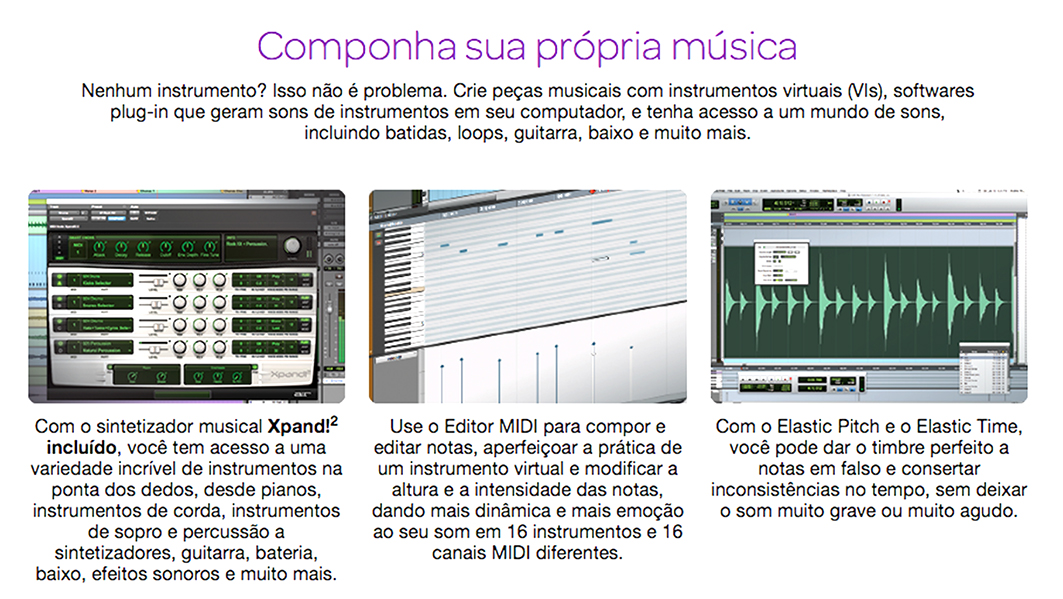
\includegraphics[width=1\linewidth]{pictures/protools}
        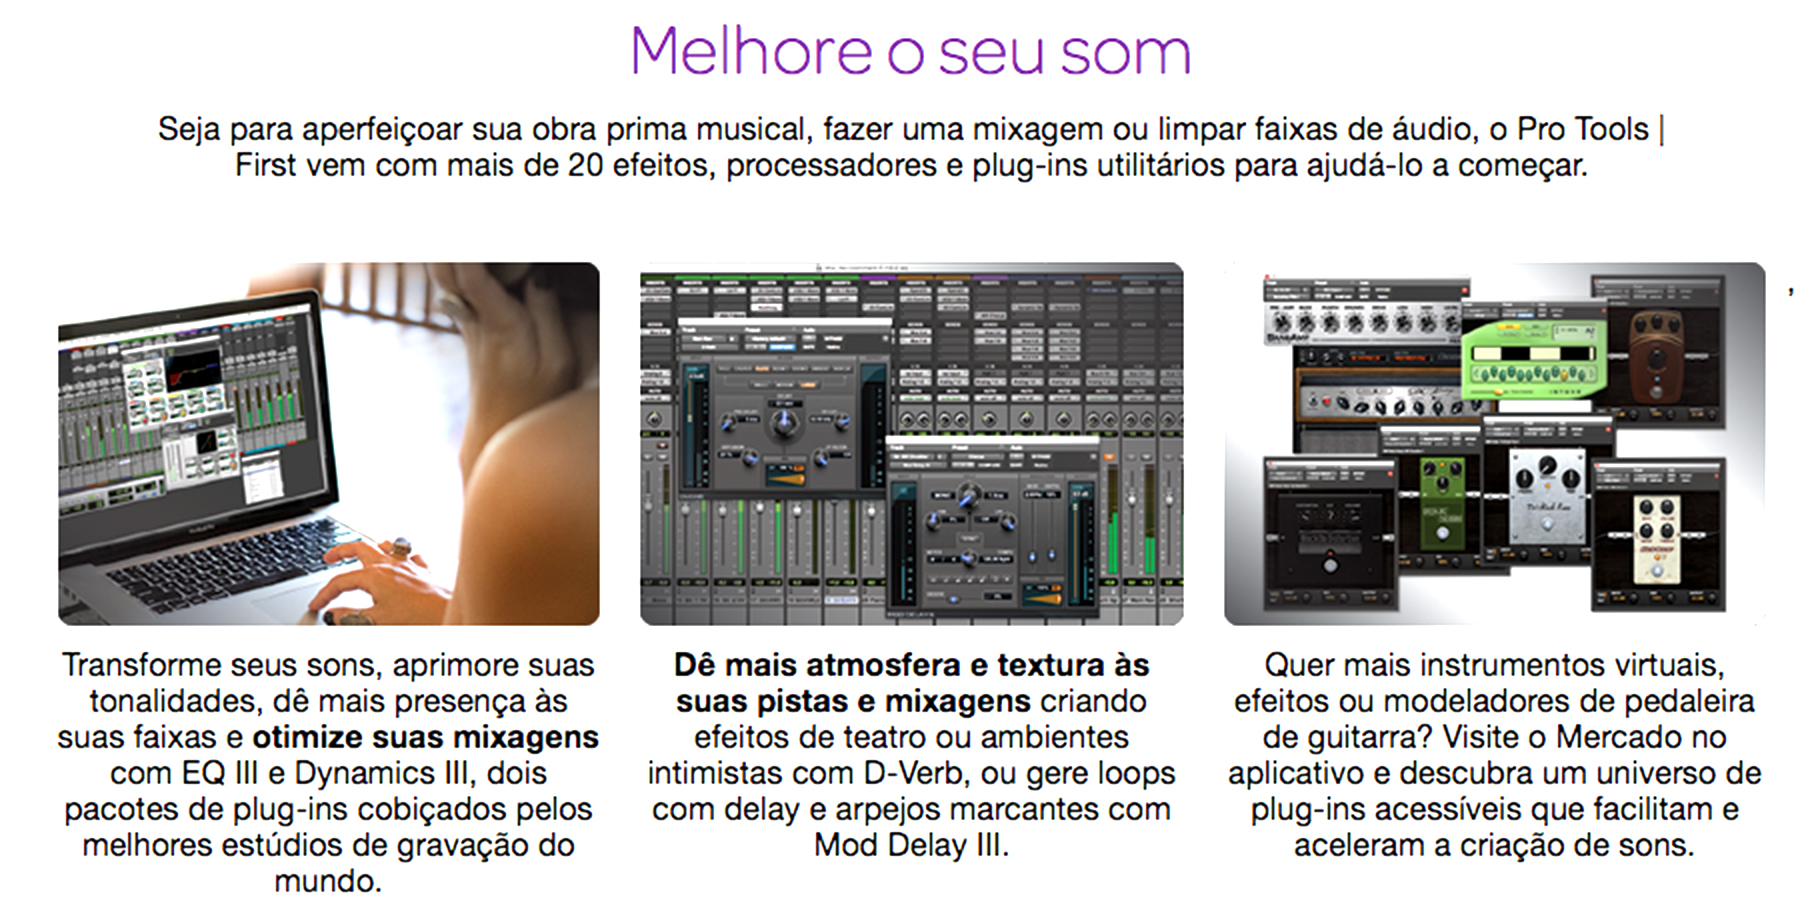
\includegraphics[width=1\linewidth]{pictures/protools2}
    \end{center}
    \legend{Fonte: Print Screen da Autora em 17 de dezembro de 2015. Site: https://www.avid.com/pro-tools-first}
\end{figure}

Outro paradigma de software voltado para produção musical é o dos programas que permitem ao usuário o design de suas próprias interfaces gráficas para controle de seus próprios aplicativos, como o Pd e o Max. Em 1986, Miller Puckette estava no IRCAN desenvolvendo um software chamado Patcher, um sistema gráfico para produção musical em tempo real para controlar a configurações de objetos no sistema MAX – um ambiente de programação orientada a objetos baseado em janelas voltado para produção musical, que na época rodava em um Macintosh, mas que já rodava no Synclavier II. O Patcher criava um sistema gráfico que simulava o sistema de cabos dos sintetizadores analógicos (figura 2) e mecanismos de abstração que permitiam condensar módulos criando entradas e saídas que poderiam ser conectadas entre si. Tratava-se na visão de Puckette, um sistema que permitiria que ``os músicos escolhessem em uma ampla gama de possibilidade, desenhando diagramas de fluxo de mensagem" \cite[5]{PucketteMiller}. 

\begin{figure}[ht]
    \caption{\label{patcher}À esquerda, um exemplo de patch feito no software Patcher de 1988, e à direita, objetos pré-programados e elementos de controle para configuração da interface gráfica.}
    \begin{center}
        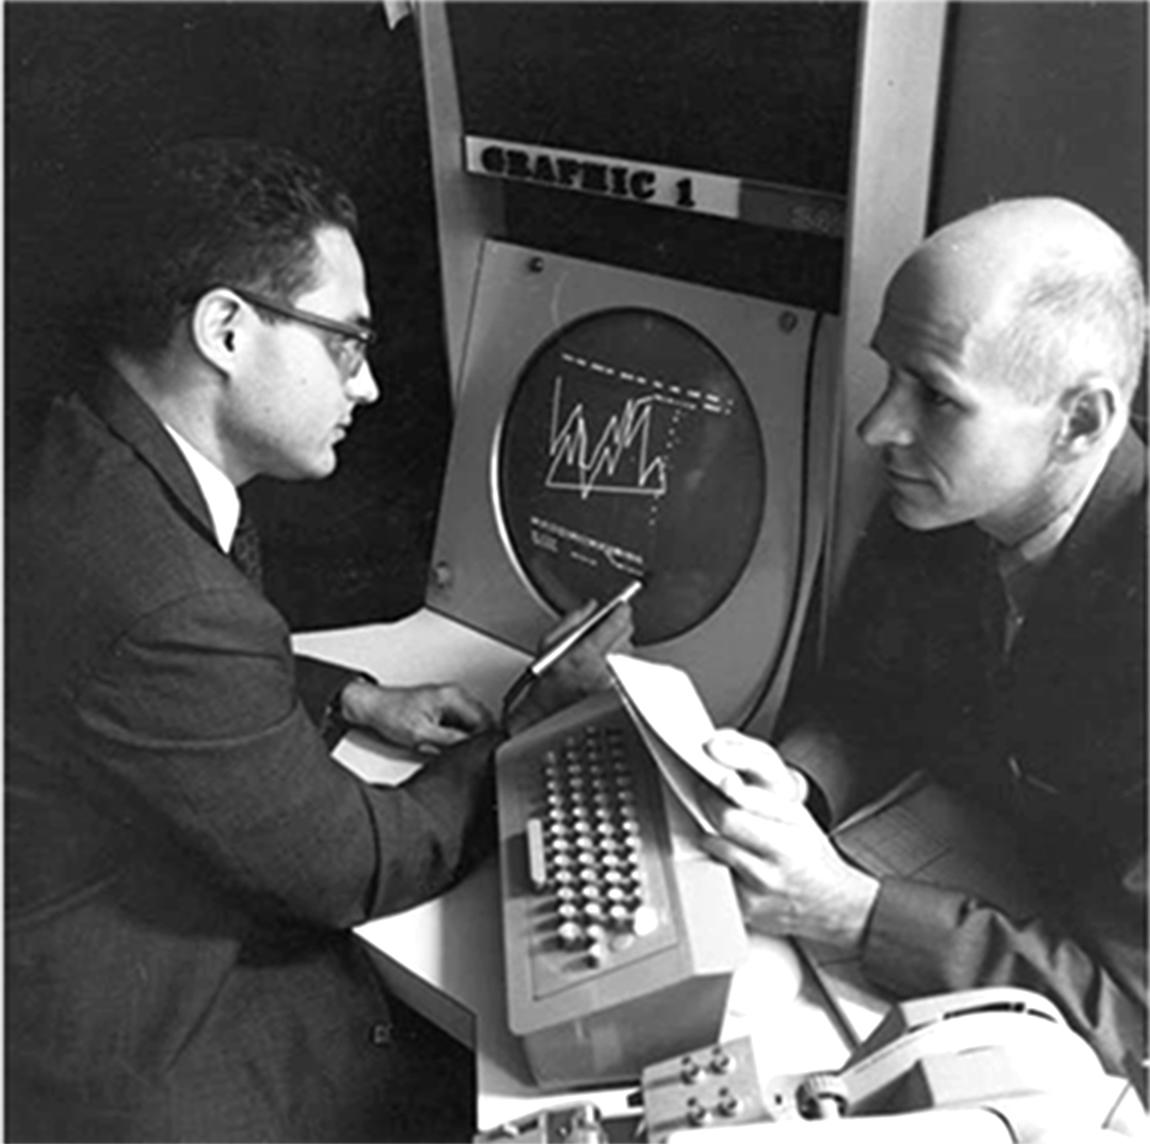
\includegraphics[width=0.5\linewidth]{pictures/MaxHolmes-251}
    \end{center}
    \legend{Fonte: \cite[6,9]{PucketteMiller}}
\end{figure}


Em 1990 o Patcher foi licenciado à Opcode e foi comercializado como Max\/Opcode, passando a ser desenvolvido por David Zicarelli. Em meados dos anos 90 a produção do software foi descontinuada pela Opcode, enquanto Miller Puckette continuou o desenvolvimento do programa no IRCAN que levou ao Max\/FTS (Faster than sound). Em 1996, Miller redesenhou totalmente o software e o lançou como um programa gratuito de código aberto chamado PureData (Pd), com uma interface gráfica muito semelhante à do Patcher original e das primeiras versões do Max. No ano seguinte, David Zicarelli fundou a Cycling 74, que continou o desenvolvimento e comercialização do Max\/MSP (abreviação tanto de Max Signal Processing ou de Miller S. Puckette) até os dias de hoje como software proprietário \cite{Cryer2018}.


Patchers, como o Pd e o Max, podem permitir a construção de interfaces complexas e adaptadas para necessidades específicas de músicos e artistas, mas possuem uma linguagem mais complexa e exigem um conhecimento especializado de quem as programa. O Pd apesar de apresentar essa modularidade também em uma metáfora de ``bancada para o design de instrumentos musicais eletrônicos para performance musical ao vivo", com objetos pré programados que podem ser conectados para que os artistas criem seus próprios instrumentos de acordo com necessidades específicas. \cite{PucketteMiller}
 
\begin{citacao}
Musicians can’t do much today without software, and so they are dependent on software developers. Software developers in turn are dependent on “users” (the musicians) to make artistic creations with their software; without that, the work of software development is pointless. The software developer strives to impose as few stylistic restrictions as possible on the musician. Yet every new generation of software that comes along reveals possibilities that were somehow not made possible, or at least not encouraged, by the previous generation. Soon we will learn that, no matter how general and powerful we believe today’s software to be, it was in fact steeped in tacit assumptions about music making that restrict the field of musical possibility. \cite{PucketteMiller}
\end{citacao}

\begin{citacao}
There is also a more subtle, and perhaps more fundamental, aim: to make it so that the software doesn’t impose one or another stylistic bias on the musician. Such a bias might be easy to spot (a built-in set of available time signatures or musical scales, for instance), or might be so ingrained as to be almost invisible (for example, Max’s and Pd’s orientation toward reactivity that seems to privilege some approaches to real-time performance over others).
\end{citacao}

\subsubsection{Interfaces para produção musical na web}
No primeiro ano desta pesquisa, além da pesquisa sobre interfaces gráficas para produção musical através de computadores, procuramos também estudar novas potencialidades que já surgiam utilizando a web como suporte.  fizemos um levantamento de experimentos organizados pelo site ``Chrome Experiments'' que reúne milhares de \emph{showcases} produzidos pela comunidade de ``programação criativa''\footnote{Disponível na url: \url{https://experiments.withgoogle.com/experiments}}. Em julho de 2016, apenas na categoria ``Sound and Music''""  haviam listados 138 experimentos. Entre experimentos estéticos com música generativa, jogos sonoros, videoclipes interativos, visualizadores de áudio, mixers e tocadores de MIDI, alguns podiam ser considerados instrumentos musicais. 

Entre eles encontramos vários exemplos de sintetizadores, samplers, processadores de áudio e sequenciadores, mas a maioria deles tinha como interface algo que mimetizava algum instrumento analógico ou eletrônico, principalmente o piano.

Encontrei algumas possibilidades interessantes como as experiências ``Lalo.li'' \footnote{Disponível em: <http://lalo.li/> }, que faz síntese de voz a partir de texto digitado na tela; ``Spectrogram and Oscillator''\footnote{Disponível em: <http://smus.com/spectrogram-and-oscillator/>}, que desenha um gráfico do espectro das frequências do som em tempo real a partir da entrada do microfone ou de um oscilador por clique ; Patatap\footnote{Disponível em: <http://patatap.com/ >}, uma espécie de bateria eletrônica audiovisual, que usa o teclado como input . Achei especialmente divertidas experiências multiusuário, como o Plink, onde cada pessoa que entra no site controlava um instrumento e vai tocando notas a partir de faixas verticais dispostas na tela (figura x) e o Multiplayer Piano\footnote{Disponível em: http://www.multiplayerpiano.com/}, um piano online aberto, que permite conexão através de midi, e tem um chat, onde diversos usuários podem tocar em uma jam coletiva ou conversarem enquanto ouvem alguém tocando.


\textbf{(ii) Instrumentos musicais online.} Nos últimos anos, principalmente depois do lançamento da Web Audio API, muitas pesquisas têm sido conduzidas no desenvolvimento de plataformas para tocar música na rede. Uma parte delas são baseadas em tipos existentes de instrumentos musicais digitais, como emuladores de DAW \cite{Jillings2017} ou sequenciadores \cite{Feenstra2016}.
\todo{incluir mais referencias aqui}

Essa diversidade de trabalhos demonstra o potencial das tecnologias web para o desenvolvimento de novas interfaces para produção musical, no entanto, a maioria dos instrumentos desenvolvidos até agora ou exigem um conhecimento prévio de técnicas musicais, ou são muitos simples e restritas em termos de expressividade musical \cite{Dobrian2006}. 


Apesar de mostraram que existe uma imensa potencialidade latente em explorar essas novas tecnologias, permitindo processos complexos de síntese de áudio e sampleamento, esses experimentos ainda são relativamente precários em termos de potencialidades de produção musical, se compararmos às ferramentas disponíveis para produção musical em software, como os chamados digital audio workstations (DAW) ou os patchers.

\end{otherlanguage*}
